% Chapitre de contribution n° 4 (TOP20 pick 4, id ED-10)
% Sources : papers/ar_yukawa_crystal/ (main.tex, AUDIT.md, REVISION.md, publication_meta.json, data/NUMERICS.md,
% data/exact_refs.jsonl, data/mpmath_control.json, gen/gen_numbers.tex), TOP20.json.
\chapter[Répulsion écrantée, erreur réparée]{La répulsion écrantée entre dans la famille du théorème, et une erreur est réparée}
\reference{Publié le 25 octobre 2026.\\ doi:10.5281/\\zenodo.23646105}

\section*{L'idée en une image}

\begin{analogie}
On sait qu'une serrure s'ouvre avec toutes les clés taillées dans une certaine ébauche. On vous tend une nouvelle
clé. Plutôt que d'essayer la porte, vous montrez, mesure à l'appui, qu'elle est taillée dans la même ébauche : elle
ouvrira donc la serrure.

\emph{Où l'image s'arrête :} la démonstration ne vaut que si la serrure fonctionne comme annoncé, c'est-à-dire si le
théorème amont est juste ; et elle dit seulement que la clé a la bonne forme, pas que le modèle physique décrit
exactement de vrais grains de poussière.
\end{analogie}

\section*{Ce qui a été fait}

Des grains de poussière chargés flottant dans un plasma, ou des billes microscopiques chargées dans un liquide
(colloïdes), se repoussent selon une loi « écrantée » : $V(r)=e^{-\kappa r}/r$, une répulsion électrique qui
s'éteint plus vite à cause du milieu environnant. Le théorème amont (chapitre précédent) s'applique à toute répulsion
qui, vue comme fonction du carré de la distance $t=r^2$, est \emph{complètement monotone} : positive, décroissante,
de pente qui s'adoucit, et ainsi de suite, les signes de toutes ses dérivées successives alternant sans fin.

Le travail prouve dans Lean que la loi écrantée a cette propriété pour tout $\kappa>0$, à toute densité, et aussi
pour tout mélange fini de telles lois avec des poids positifs (par exemple deux populations d'ions qui écrantent à des
distances différentes). Si le théorème amont est juste, le réseau triangulaire est donc l'arrangement d'énergie
minimale pour ces systèmes. Les mathématiques sont classiques ; ce qui est nouveau, c'est que ces conséquences sont
écrites et contrôlées par la machine.

\begin{encadre}
\textbf{À faire avec un crayon (et une calculatrice).} Prenons $\kappa=1$ et $g(t)=e^{-\sqrt t}/\sqrt t$. On trouve
$g(1)=e^{-1}\approx0{,}368$, $g(4)=e^{-2}/2\approx0{,}068$, $g(9)=e^{-3}/3\approx0{,}017$. Les valeurs descendent
(première condition de signe), et les descentes rétrécissent : $0{,}300$ puis $0{,}051$ (deuxième condition). Ce ne
sont que deux conditions parmi une infinité ; la machine les vérifie toutes, pour tout $t>0$.

\textbf{Pourquoi les poids doivent être positifs.} Le mélange $g_1-2g_2$ (une loi moins deux fois une loi plus
écrantée) vaut, en $t=1/4$, $2e^{-1/2}-4e^{-1}\approx1{,}213-1{,}472=-0{,}258$. Il est négatif : il échoue dès la
première condition, et le théorème ne s'applique pas à lui. Attention : cela ne prouve pas que les triangles perdent
pour ce mélange ; la question reste ouverte.
\end{encadre}

Le même article répare l'erratum du chapitre précédent. La simulation du 11 octobre coupait la force au-delà d'une
distance $r_c=8$, avec une correction dite « à force décalée ». La figure~\ref{fig:c04} recalcule le prix de cette
coupure : à $\kappa=1$, l'énergie de chaque arrangement était sous-estimée d'environ $0{,}0177$, presque deux fois
l'écart de $0{,}0095$ entre réseau carré et réseau triangulaire. Avec la loi exacte, sans coupure, et une borne
rigoureuse sur la queue de la somme, l'énergie du réseau triangulaire passe de $1{,}6076$ à $1{,}6253$. Mais le
décalage touche toutes les configurations presque de la même façon : l'écart carré--triangle ne bouge que de
$-2{,}2\times10^{-6}$. Les 24 configurations publiées qui ont été relaxées de nouveau avec la loi exacte restent
toutes au-dessus du réseau triangulaire, à la précision de l'ordinateur près ; l'une d'elles est le réseau parfait
lui-même, à écart nul.

\begin{figure}[htbp]
\centering
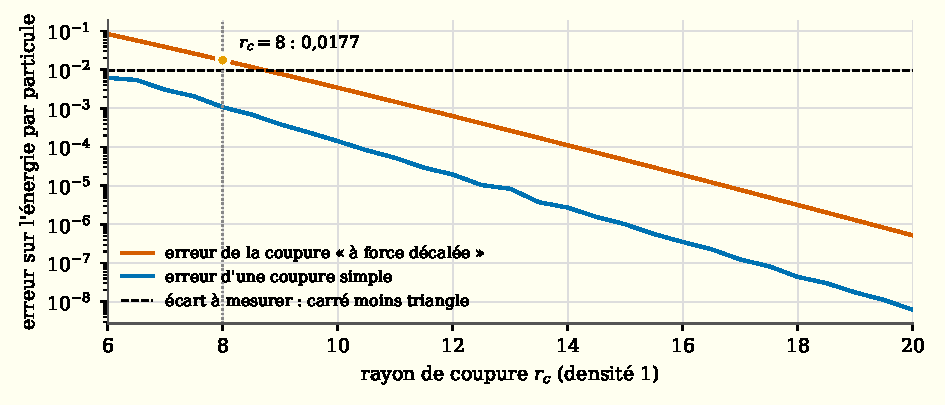
\includegraphics[width=\linewidth]{figures/c04_coupure}
\caption{Erreur sur l'énergie par particule du réseau triangulaire ($\kappa=1$) selon le rayon de coupure, recalculée
par sommes directes et comparée à l'écart carré--triangle.}
\label{fig:c04}
\end{figure}

\section*{Comment on s'est assuré que ce n'est pas faux}

\niveau{A} \emph{Le juge a regardé.} Lean, le programme qui contrôle chaque pas d'une preuve, a accepté les deux
fichiers avec seulement les trois hypothèses de base admises partout ; une preuve laissée en blanc et un axiome
inventé, plantés exprès, ont été détectés ; les deux modules ont été rejoués sans erreur par un second programme de
contrôle le 26 octobre 2026. Un agent d'IA indépendant a recompilé des copies exactes des fichiers, planté ses propres
pièges, vérifié pas à pas la démonstration écrite pour les humains, et rendu un avis favorable avec cinq corrections de
formulation, toutes appliquées ; aucun énoncé ni aucun nombre n'a changé. Comme partout dans ce livre, aucun humain
spécialiste n'a relu ces résultats, et le registre des affirmations le signale par 11 drapeaux.

Pour les calculs \niveau{X}, un contrôle indépendant à 40 chiffres (une autre méthode, un autre code) retrouve les
énergies exactes à $1{,}7\times10^{-16}$ près. Le test fait pour échouer échoue : les anciennes valeurs à force
décalée ne passent pas le contrôle d'accord. Et le réseau carré reste un col instable sous la loi exacte.

\section*{Ce que ça ne dit pas}

\begin{limite}
\begin{itemize}
\item Tout dépend du théorème amont, produit par une IA et non encore relu par des pairs.
\item La loi étudiée est la répulsion écrantée en trois dimensions, restreinte au plan ; la loi d'écrantage purement
bidimensionnelle n'est pas traitée.
\item Rien sur la température, la fusion, ni le chemin par lequel un vrai système atteint le réseau.
\item Les nouvelles relaxations couvrent un sous-ensemble de l'étude publiée (11 sur 50 à $\kappa=1$, 13 sur 100 à
$\kappa=2$), et le recuit n'a pas été refait.
\end{itemize}
\end{limite}

\section*{Pour aller plus loin}

C'est une correction menée jusqu'au bout : l'erreur d'un article est réparée dans un autre, à l'intérieur de la même
boucle auditée. Article : doi:10.5281/zenodo.23646105.
